\section{Einleitung}
Die Firma ARM bietet eine breite Palette von Prozessoren, hierbei ist zu sagen das im Laufe der Zeit verschiedene Versionen, wie ARMv1-ARMv8, in Betrieb waren. Diese Versionen beziehen sich nicht auf einen speziellen Prozessor sondern definieren eine Spezifikation auf deren Basis ein Prozessor, wie f\"ur diese Bachelorarbeit der ARM926EJ-S in der Version ARMv5. F\"ur die Bachelorarbeit wurde die ARMv5 gew\"ahlt weil diese Prozessoren in vielen Handheld verbaut werden und im gegenteil dazu die Rechenkraft eines ARMv7 nicht ben\"otigt wurde.
\begin{table}[h!]
\centering
\begin{tabular}{|l|c|c|}
\hline
Version & Beispielprozessor & Beispielverwendung \\ \hline
ARMv1 (1985) & ARM1 & BBC Master \\ \hline
ARMv2 (1986) & ARM2, ARM3 & Acorn-Archimedes \\ \hline
ARMv3 (1991) & ARM6, ARM7 & Apple Newton, RISC PC \\ \hline
ARMv4 (1995) & ARM7TDMI, ARM8 & Gameboy Advanced, Nintendo DS \\ \hline
ARMv5 (1997) & ARM7EJ, \textbf{ARM926EJ-S} & Palm Tungsten \\ \hline
ARMv6 (2002) & ARM11, ARM-Cortex-M0 & nvidia, Texas Instruments \\ \hline
ARMv7 (2004) & ARM-Cortex-M1 & nvidia, Texas Instruments  \\ \hline
ARMv8 (2014) & ARM Cortex-A50 & Mobilefunktger\"ate, Tablets \\ \hline
\end{tabular}\vspace{0.5cm}
\footnotesize\textbf{Quelle:}\url{https://de.wikipedia.org/wiki/ARM-Architektur#Modelle},Letzter Aufruf: 24.07.2013
\caption{Unterschiedliche ARM Versionen}
\end{table}
\newpage
\section{RISC- vs CISC-Prozessoren}
Der Begriff ARM bedeutet \textit{Advanced RISC Machine}. Hier muss jedoch ein weiterer Begriff herausgezogen werden, RISC. RISC bedeutet \textit{Reduced Instruction Set Computer}, der Begriff \textit{Reduced} bezieht sich jedoch nicht auf einen kleineren Instruktionssatz sondern mehr auf die Komplexit\"at der Instruktionen selbst. Die Instruktionen bei einer RISC Maschine sind wesentlicher einfacher als die einer CISC. So ist es deshalb m\"oglich das Chipdesign zu vereinfachen. Durch das einfachere Chipdesign k\"onnen mehr Register auf den Chip gebracht werden und die Performance von Operationen ist h\"oher. Die Daten k\"onnen in  Register geladen und die Performanceintensiven Speicherzugriffe reduziert werden. Daraus l\"asst sich doch schlie\ss en das sich RISC eigentlich gegen\"ueber CISC auf dem Markt h\"atte durchsetzen m\"ussen. Doch das war nicht so. Warum? Tanenbaum hat dazu in seinem Buch \"uber \textit{Structured computer organisation} folgende geschrieben: 
\begin{quote}
\blockquote{\textit{First of all, there is the issue of backward compatibility and the billions of
dollars companies have invested in software for the Intel line. Second, surpris-
ingly, Intel has been able to employ the same ideas even in aCISC architecture.}}
\end{quote}\parencite[80]{tane:sco} \\\\
Im Gegenteil dazu stehen die CISC Maschinen - \textit{Complex Instruction Set Computer}. Diese Familie der Computer ist die wohl am weitesten verbreitete Technologie am Markt. Chipdesigner wie Intel und AMD bauen zum gro\ss teil diese Architekturen. Ein CISC hat im Gegenteil zu einem RISC ein weitaus kleineren Instruktionssatz, aber daf\"ur ist die Komplexit\"at h\"oher. Dadurch wird erreicht, dass mit weniger Befehlen umfangreiche Operationen durchgef\"uhrt werden k\"onnen. Der Nachteil dabei ist jedoch das die Performance, der Befehlsausf\"uhrung, geringer als bei einem RISC ausfallen kann.
\begin{table}[h!]
\centering
\begin{tabular}[h!]{|p{4cm}|p{4cm}|p{5cm}|}
	\cline{1-3} 
	& \textbf{RISC} & \textbf{CISC} \\ \hline 
	\textbf{CPU Zyklen pro \newline Instruktion} & wenig Zyklen pro Instruktion & mehrere Zyklen \\ \hline
	\textbf{Komplexit\"at der \newline Instruktionen} & wesentlich geringer & hoch bis sehr hoch\\ \hline
	\textbf{Umfang Instruktionssatz} & hoch & gering \\ \hline
	\textbf{Instruktions-\newline geschwindigkeit} &  hoch bis sehr hoch & gering \\ \hline
	\textbf{Verwendung}  & Smartphones, Tablets und andere Ger\"ate die wenig Energie verbrauchen sollen. & Computer \\ \hline	 
	
\end{tabular}
\caption{Vergleich RISC vs. CISC}
\end{table}
\\
\noindent
Fazit dieses Vergleiches ist dass, beide Architekturen ihre Da-Seins Berechtigung in der aktuellen Technologischen Welt haben. Beide Versionen bringen Vor- und Nachteile mit sich, aber einen echten Gewinner gibt es in dem Spiel nicht. CISC machen sich viele Mechanismen der RISC zu nutze und n\"ahern sich ihnen so immer mehr an. Jedoch wird sich RISC niemals in der Welt der Heim-Computer durchsetzen aber immer Vorreiter im Bereich Embedded Systemen bleiben.
\section{ARM926EJ-S}
Betriebssysteme lassen sich auf jeder Prozessorarchitektur entwickeln die man sich vorstellen kann. Die Wahl auf den ARM926EJ-S fiel aufgrund diverser Recherchen. Aufgrund der Tatsache das es f\"ur die g\"angigen Intel und AMD Prozessoren bereits weitverbreitete Betriebssysteme gibt fiel die Wahl im vorhinein nicht auf diese Art.\\
Nach dem klar war wo ARM-Prozessoren eingesetzt werden, wie z.B. in Druckern, Handys, Tablets und vielen mehr, fiel die Entscheidung auf diesen Prozessor. Zudem kommt hinzu es gibt momentan noch nicht so viele Betriebssysteme wie bei den anderen Systemen. Vorteile sind z.B.
\begin{dinglist}{227}
	\item{\textbf{Energieeffizienz}}
	\item{\textbf{Schnelligkeit}}
	\item{\textbf{geringe Produktionskosten}}
	\item{\textbf{minimale Bauweise.}}
\end{dinglist}
\section{Register}
Der ARM926 Prozessor ist ein 32-Bit RISC Prozessor. Dieser Prozessor hat eine Gesamtzahl von 37 Registern\parencite[vgl.][44\psqq]{archManI}, wobei 30 dieser Register den allgemeinen Zwecken und 6 als Statusregister dienen. Von diesen hier explizit die Register \textbf{R0-R7} und \textbf{R13-R15} zu erw\"ahnen sind. \textbf{R0-R7} sind tats\"alich allgemein verwendbare Register, die unabh\"angig von dem aktuellen Prozessormodus sind, \textbf{R13} ist der \textit{Stackpointer}, \textbf{R14} stellt das \textit{Linkregister} dar und \textbf{R15} bezeichnet den \textit{Program Counter}.
\begin{dinglist}{227}
	\item{\textbf{Stackpointer}}\\
	Zeigt auf die 'Top-Of-Stack' Adresse
	\item{\textbf{Linkregister}}\\
	Zeigt auf den aktuell geretteten Programmcounter bevor eine Routine betreten wird
	\item{\textbf{Programmcounter}}\\
	Zeigt auf die n\"achste Instruktion
\end{dinglist}
\begin{figure}[H]
\center
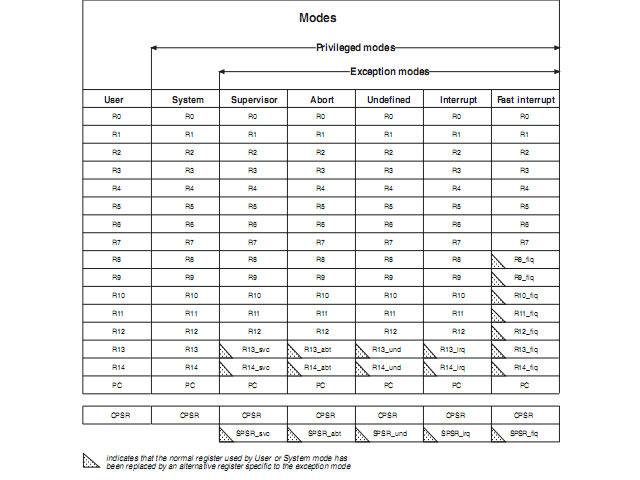
\includegraphics[scale=0.7]{common/register.png}\\
\footnotesize\textbf{Quelle:}\parencite[43]{archManI}
\caption{ARM926EJ-S Register}
\end{figure}
Teilweise sind die Register mehrfach vergeben, denn im ARM Prozessor gibt es unterschiedliche Prozessor-Modi und f\"ur ein Gro\ss teil dieser Modi stellt der Prozessor f\"ur R13 und R14 neue Register zur Verf\"ugung. Das spielt dann eine wichtige Rolle, wenn man unterschiedliche Stacks f\"ur die Modi aufbauen muss.
\section{Prozessor Modus}
Der ARM926EJ-S stellt sieben unterschiedliche Modi bereit, in der sich der Prozessor befinden kann. Jeden dieser Modi kann man per Programmcode oder durch einen Interrupt betreten. 
\begin{dinglist}{227}
	\item{\textbf{User} \\ Das ist der Modus, in dem alle Benutzerprogramme laufen. Sie haben keinen direkten Zugriff auf die Kernel-Routinen, sondern m\"ussen daf\"ur Trap-Instruktionen benutzen.}
	\item{\textbf{FIQ(extra R8-R14) }\\ Dieser Modus wird nur von sehr wenigen Interrupts betreten. Das sind die Interrupts, die eine sehr hohe Priorit\"at haben und umgehend von dem Prozessor behandelt werden m\"ussen.}
	\item{\textbf{IRQ(extra R13-R14)}\\ Alle Standard Interrupts, wie Tastatureingabe und andere, die darauf konfiguriert werden, landen in diesem Modus. Routinen in diesem Modus k\"onnen in den User-Modus wechseln, um User-Programme auszuf\"uhren.}
	\item{\textbf{Supervisor(extra R13-R14)} \\ Dieser Modus ist ausschlie\ss lich f\"ur Trap-Routinen reserviert. Das bedeutet, alle Instruktionen, die von einem Userprogramm aufgerufen wurden, um Kernel-Methoden auszuf\"uhren.}
	\item{\textbf{Abort(extra R13-R14)}\\ Abort ist der Modus, in den der Prozessor f\"allt, wenn entweder eine Instruktion aufgrund eines Fehlers abgebrochen werden muss oder ein Fehler beim Abruf einer Speicherstelle auftritt.}
	\item{\textbf{Undefined(extra R13-R14)}\\ Dieser Modus wird nur dann betreten, sofern der ARM-Prozessor eine Instruktion von einem Co-Prozessor anfordert, dieser aber nicht reagiert.}
	\item{\textbf{System} \\ Dieser Modus ist nur f\"ur den Kernel. Kein User-Programm darf diesen betreten.}
\end{dinglist}
Der System-Mode ist ein spezieller Modus. Dieser wird \"uber keinen Interrupt ausgel\"ost. Er ist deshalb vorhanden, weil das Betriebssytem ihn benutzt, um Betriebssytem-relevante Resourcen zu benutzen. Weiterhin verf\"ugt dieser Modus die gleichen Register wie der User-Modus.
\section{Interrupt-Controller}
Der ARM926EJ-S besitzt einen speziellen Interrupt-Controller, den sogenannten \textit{Vectored Interrupt Controller - VIC}. Das ist eine Hardwarekomponente, die ein System zwischen Interrupts und dem Betriebssystem darstellt. Jede Hardware muss auf einem Chip an eine bestimmte Adresse gelegt werden. F\"ur den VIC gibt es folgende Spezifikation:
\begin{figure}[H]
\center
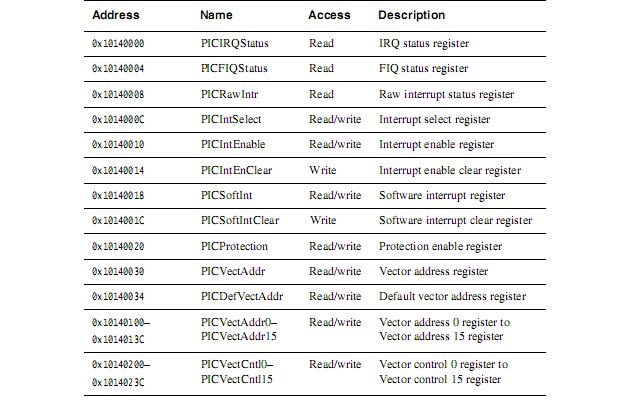
\includegraphics[scale=0.7]{common/processor-vic.png}\\
\footnotesize\textbf{Quelle:}\parencite[224]{archManI}
\caption{VIC Register}
\end{figure}
\noindent
Der Entwickler hat nun die M\"oglichkeit, diese Adresse programmatisch anzusteuern, um Informationen aus dem VIC zu erhalten. Die f\"ur dieses Projekt wichtigsten Register sind Folgende:
\begin{dinglist}{227}
	\item{\textbf{IRQ/FIQ Status Register - 0x10140000/0x10140003}}\\
	Mit diesem Register kann ermittelt werden, wie der aktuelle Status eines IRQ/FIQ ist.
	\item{\textbf{Select Register - 0x01014000C}} \\
	Mit diesem Register kann bestimmt werden , welcher Interrupt ein IRQ oder FIQ sein soll.
	\item{\textbf{Interrupt enable register - 0x10140010}} \\
	Gibt an, ob ein bestimmter IRQ/FIQ von dem VIC beachtet werden soll.
	\item{\textbf{Interrupt enable clear register - 0x10140014}}\\
	Mit diesem Register kann ein Interrupt nach Ausl\"osung geleert werden.
	\item{\textbf{Vector address register - 0x10140030}}\\
	In dieses Register schreibt der VIC die Adresse der Interrupt Service Routine des momentan ausgel\"osten Interrupts.
	\item{\textbf{Vector address register 0 - 15 - 0x10140100-0x1014013C}}\\
	In diese Register m\"ussen die Adressen von den Interrupt Service Routinen geschrieben werden, die f\"ur diesen Interrupt zust\"andig sind.
	\item{\textbf{Vector control register 0 - 15 - 0x10140200-0x1014023C}}\\
	In diese Register muss man \"aquivivalent zu den 'Vector address registern' die Quelle des Interrupts und, ggf. ob der Interrupt aktiviert werden soll, schreiben.
\end{dinglist}